\chapter{Анализ предметной области}
\label{ch:chap1}

\section{Автономная навигация}
Задача навигации является основопологающей при функционировании мобильного робота. 

Автономная навигация - это способность робота воспринимать информацию о внешнем мире через датчики, строить по этим данным модель окружения, оценивать свою конфигурацию в этом окружении, строить достижимую траекторию движения до заданной цели навигации и подавать такое управление на моторы, которое способствовало бы движению по построенной траектории. \\
Автономность навигации заключается в том, что планировщик траектории, являющийся частью системы навигации робота, может без вмешательства человека-оператора формировать путь до цели, учитывая объезд препятствий.

Исходя из данного определения задачу автономной навигации можно разделить на 4 отдельных подзадачи:
\begin{itemize}
    \item восприятие окружения;
    \item локализация робота и построение карты местности;
    \item планирование пути;
    \item управление движением.
\end{itemize}
На Рисунке \ref*{fig:navigation_diagram} представлена диаграмма задачи навигации, на ней можно увидеть как компоненты систему связаны между собой.

\begin{figure}[h]
    \centering
    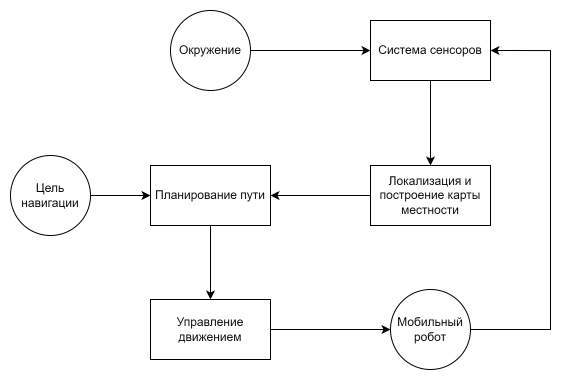
\includegraphics[width=0.75\textwidth]{images/chap_1/navigation_diagram.png}
    \caption{Диаграмма задачи навигации}
    \label{fig:navigation_diagram}
\end{figure}

Любая система для автономной навигации мобильного робота реализует в какой-то форме данные компоненты. Архитектуры таких систем принято выполнять в иерархичной структуре, соответствующей парадигме "Ощущать, думать, действовать" 
 \cite{murphy2019introduction}.

\begin{figure}[h]
    \centering
    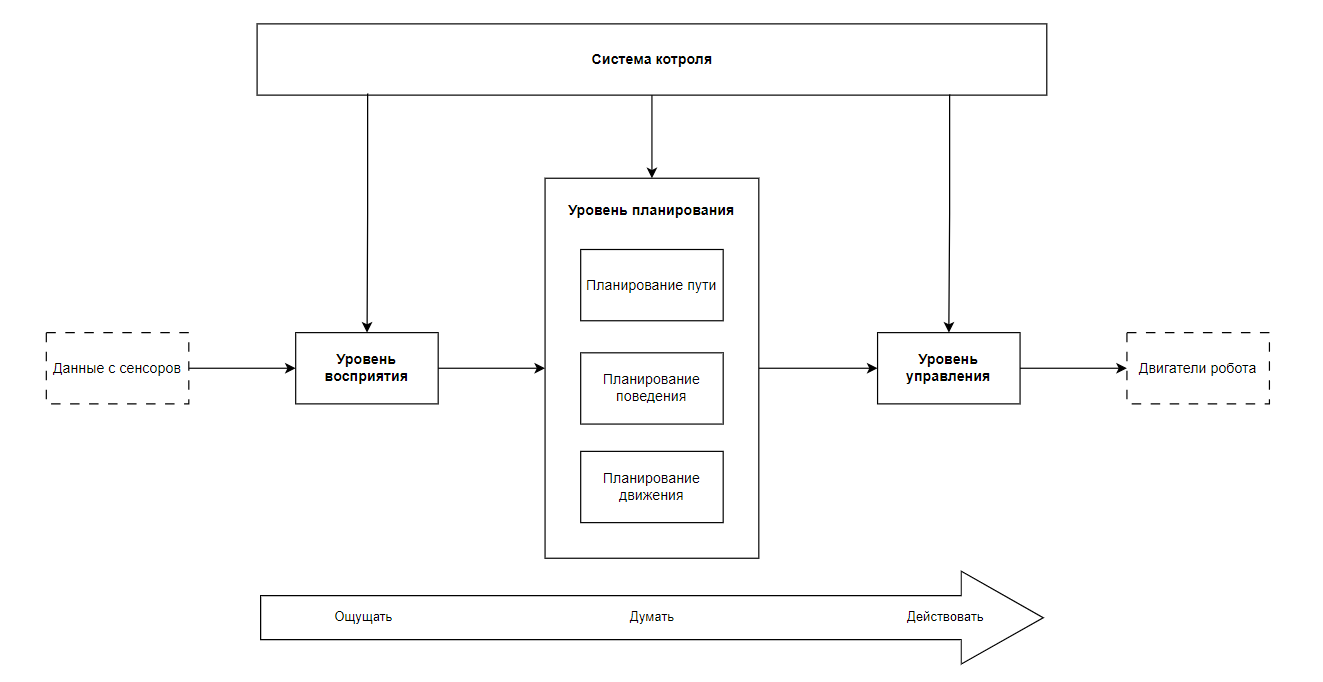
\includegraphics[width=1.0\textwidth]{images/chap_1/sense_think_act.png}
    \caption{Диаграмма стандартной архитектуры системы автономной навигации робота}
    \label{fig:sense_think_act}
\end{figure}

Структура данной архитектуры представлена на Рисунке \ref*{fig:sense_think_act}. \\
На уровне восприятия происходит анализ данных с сенсоров и соответствующая локализация и построение карты местности, а на уровне управления - непосредственная подача сигналов на двигатели робота. \\
Рассмотрим подробнее уровень планирования. Как видно, он разделен на 3 компонента:
\begin{itemize}
    \item планирование пути (глобальный планировщик) - реализует построение траектории движения робота от его начальной точки до конечной;
    \item планирование поведения - выполняет задачу по корректировке траектории, построенной глобальным планировщиком, в соответствии с локальным состоянием окружения (объезд появившихся препятствий, в том числе динамических, следование правилам движения и заданным ограничениям);
    \item планирование движения (локальный планировщик) - основной задачей является исполнение задачи слежения за траекторией, полученной от поведенческого слоя.
\end{itemize}
Также важным компонентом такой архитектуры является система контроля. Она обрабатывает информацию о состоянии всех компонентов и производит проверки для определения неполадок во время функционирования системы. В случае если была обнаружена неисправность или нежелательное поведение системы, модуль контроля обеспечивает приостановку нормального функционирования системы и делает попытки по восстановлению её работоспособности. Это позволяет повысить безопасность и автономность системы.

В последующих секциях данной главы мы разберем подробнее подзадачи навигации и представим современные способы их решения.

\subsection{Восприятие окружения}
Системы восприятия окружения позволяют роботу получать информацию об окружающей его среде. Получаемая информация может иметь разнообразный вид, исходя из этого все системы можно разделить на следующие группы \cite{yurev_sensors}:
\begin{enumerate}
    \item Системы, определяющие геометрические и другие параметры окружения. Такие системы позволяют получить данные о пространсвенном расположении, расстоянии, форм и размеров объектов в окружении. Выходные данные системы представлены в простой форме (например, расстояние до объекта в метрах), а значит анализ информации не требует больших вычислительных ресурсов, а используемые алгоритмы имеют относительно небольшую пространственную и вычислительную сложность. Примерами таких систем являются лазерные дальномеры (LIDAR), ультразвуковые дальномеры (SONAR), акселерометры, одометры, камеры глубины и другие  
    \item Системы компьютерного зрения. Единицей информации в таких системах - изображение с камеры, поступающие с определенной частотой. Этап обработки таких данных обычно подразумевает выделение характеристик или свойств, которые будут использованы для выполнения задачи навигации. Стоит отметить, что алгоритмы технического зрения требуют больших вычислительных мощностей
    \item Системы силомоментного очувствления роботов. Данные системы основаны на измерении сил и моментов сил. Получение обратной связи от окружения в форме силовых покателей может быть важным аспектом системы навигации. Примером такой системы для мобильного робота является датчик столкновения 
    \item Системы, использующие несколько различных типов сенсоров. Применение разных видов датчиков позволяет получать данные разной природы и обеспечивает избыточность данных. Однако в таком случае появляется необходимость решать задачу объединения данных
\end{enumerate}

\subsection{Локализация и построение карты местности}
Задача SLAM является важной частью в автономной навигации робота. Алгоритмы SLAM принимают на вход данные с различных сенсоров робота (в основном камеры, лазерные дальномеры и инерциальные измерительные приборы), производят из обработку и объединение. Результатом их работы является карта окружения с отмеченным положением робота на ней. \\
Алгоритмы SLAM можно разделить на 2 группы \cite{barfoot2024state}:
\begin{enumerate}
    \item Визуальный SLAM - использует изображения с камер. Применяемые алгоритмы: PTAM, ORB-SLAM, DTAM, DSO
    \item Лазерный SLAM - использует данные с лазерных дальномеров. Применяемые алгоритмы: ICP, NDT, LOAM, FGR
\end{enumerate}

Однако на практике локализация и построение карты местности производится с использованием нескольких сенсоров. Это позволяет существенно увеличить точность и надежность SLAM, так как преимущества отдельных датчиков складываются, а индивидуальные недостатки сглаживаются.

\subsection{Планирование пути}
Планирование пути – поиск последовательности конфигураций робота для передвижения его из точки A в точку Б.  \\
На задачу планирования пути оказывают влияние следующие факторы:
\begin{itemize}
    \item габариты, кинематические и динамические ограничения робота;
    \item тип окружения (статическое или динамическое);
    \item наличие карты местности (существует заранее созданная карта местности или же используется SLAM);
    \item степень неопределенности при работе сенсоров (зашумленная или неполная информация) и при передвижении робота;
    \item требования к используемому алгоритму:
    \begin{itemize}
        \item вид функционала качества;
        \item пространственная и временная сложности;
        \item точность решения.
    \end{itemize}
\end{itemize}

\subsubsection{Математическое описание задачи}
Конфигурация робота - минимальное множество параметров, которые определяют степени свободы робота относительно фиксированной системы координат. В данной работе мы рассматриваем двумерную систему координат, тогда конфигурация будет иметь вид:
\begin{equation}
    \label{eq:e1}
    q = (x, y, \theta).
\end{equation}
Конфигурационное пространство $C$ - пространство всех возможных конфигураций робота:
\begin{equation}
    \label{eq:e2}
    C: \mathbb{R}^2 \times SO(2).
\end{equation}
Конфигурационное пространство разбивают на 2 непересекающихся множества:
\begin{equation}
    \label{eq:e3}
    C = C_\textup{преп} \cup C_\textup{своб}, \qquad C_\textup{преп} \cap C_\textup{своб} = \emptyset. 
\end{equation}
\begin{figure}[h]
    \centering
    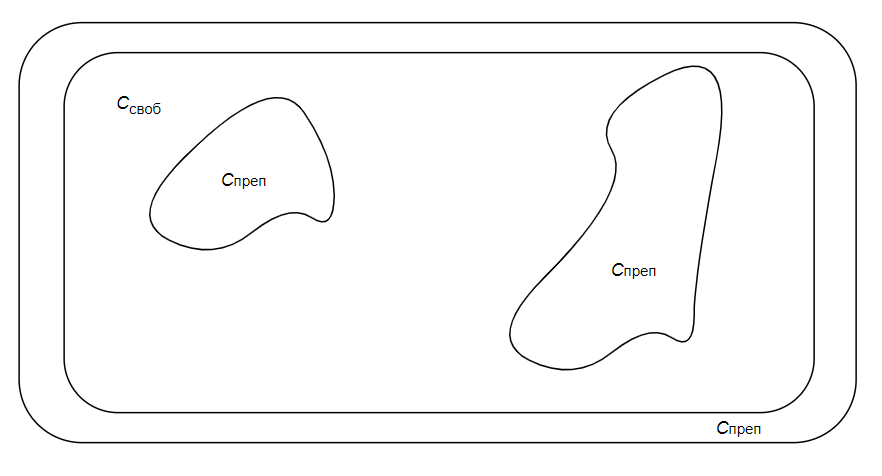
\includegraphics[width=0.75\textwidth]{images/chap_1/conf_space.png}
    \caption{Конфигурационное пространство}
    \label{fig:conf_space}
\end{figure}
На Рисунке \ref*{fig:conf_space} представлен пример разбиения конфигурацинного пространтсва. \\
Тогда задачу планирования можно представить в форме поиска непрерывного пути:
\begin{equation}
    \label{eq:e4}
    \tau : [0,1] \rightarrow C_\textup{своб}, \qquad \tau(0) = q_\textup{старт}, \qquad \tau(1) = q_\textup{цель}.
\end{equation}

\subsubsection{Классификация алгоритмов планирования}
Приведем основные виды алгоритмов планирования пути \cite{lavalle2006planning}:
\begin{enumerate}
    \item На основе графов: диаграмма видимости, диаграмма Вороного, вероятностная дорожная карта, метод быстро исследующих случайных деревьев (RRT)
    \item На основе клеточной декомпозиции: алгоритмы Дейкстры, A*, D*
    \item На основе потенциальных полей
    \item Оптимизационные методы
    \item На основе интеллектуальных технологий: муравьиный алгоритм, ANN, метод роя частиц, реактивные методы
\end{enumerate}

\subsection{Управление движением}
Управление движением решает задачу перевода высокоуровеных задач навигации в конкретные сигналы управления, подаваемые непосредственно на двигатели робота. \\
В данной задаче можно выделить 3 основных аспекта:
\begin{enumerate}
    \item Задача слежения
    \item Наличие обратных связей управления
    \item Учет ограничений робота
\end{enumerate}

Способность реализовывать намеченный план передвижения является основополагающей в задаче навигации. Для решения задачи слежения применяются методы теории автоматического управления.

Дадим математическое описание задачи слежения \cite{math-control-theory}. \\
Пусть $y(t)$ - выходной сигнал замкнутой системы, $g(t)$ - эталонный сигнал, $u(t)$ - сигнал управления. Тогда целью управления задачи слежения будет:
\begin{equation}
    \label{eq:e5}
    \lim _{t \rightarrow \infty} (y(t)-g(t)) = 0.
\end{equation}

\begin{figure}[h]
    \centering
    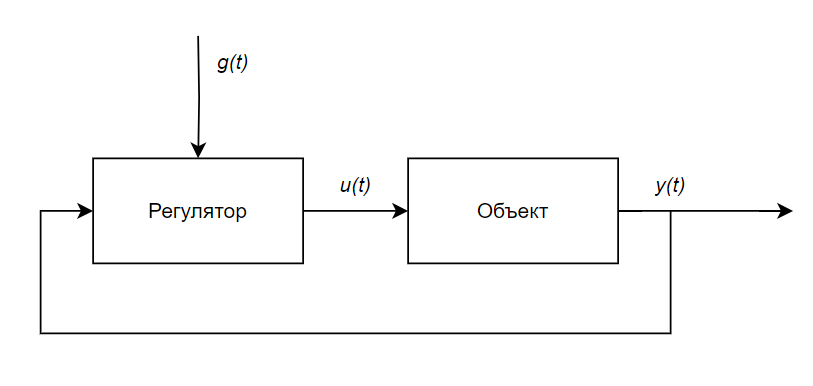
\includegraphics[width=0.75\textwidth]{images/chap_1/tracking_scheme.png}
    \caption{Блок-схема системы управления выполняющей слежение за эталонным сигналом}
    \label{fig:tracking_scheme}
\end{figure}

Итак, при решении задачи слежения используются методы управления с обратной связью, которые на основе данных с сенсоров корректируют траекторию движения мобильного робота. Использование ПИД-регулятора является одним из наиболее простых решений для данной задачи. 

\section{Методы принятия решений}
Методы принятия решений представляют собой системы, который на высоком уровне решают, какая стратегия поведения робота будет выполняться на основе данных о состоянии робота и его окружения. Все описанные ниже системы принятия решений основаны на использовании состояний, в который может находиться робот. 

\subsection{Конечный автомат}
Конечные автоматы описывают поведение в форме состояний, которые вызывают выполнение соответствующих действий. Используя конечный автомат можно разделить задачу управления на отдельные блоки, получив наглядное представление того, в каких случаях система будет оказываться в определенном состоянии. \\
Такая структуризация упрощает дальнейшую отладку (например, если робот застрял в определенном состоянии, легко определить, какой переход или какое условие не работает). 

\begin{figure}[h]
    \centering
    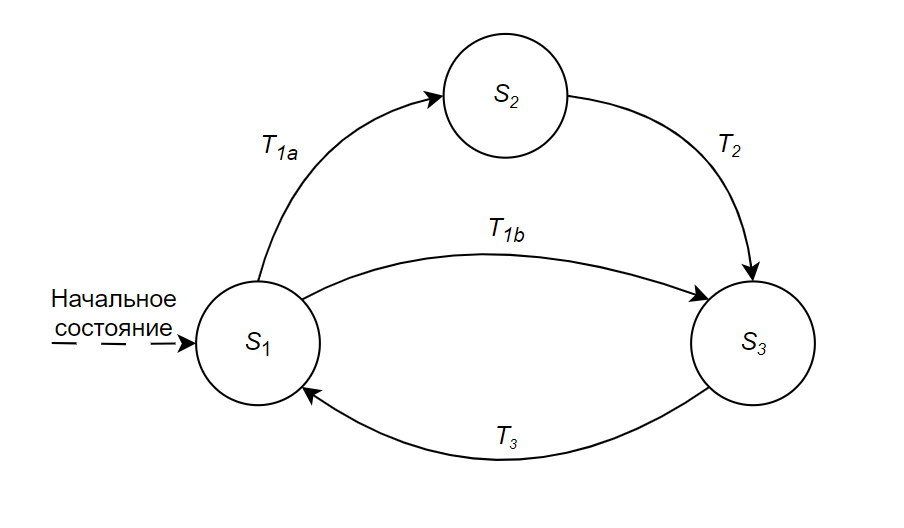
\includegraphics[width=0.75\textwidth]{images/chap_1/fms.png}
    \caption{Графическое представление конечного автомата}
    \label{fig:fms}
\end{figure}

На Рисунке \ref*{fig:fms} представлено графическое описание конечного автомата, состоящее из дискретных состояний, представленных узлами графа, и переходов, представленных ребрами. Когда срабатывает переход, конечный автомат изменяет свое текущее состояние и совершает переход в другое состояние в соответствии с функцией перехода.

В математической форме конечный автомат имеет вид кортежа \cite{wagner2006modeling}:
\begin{equation}
    \label{eq:e6}
    A = (S, \Sigma, \delta, s_0, F).
\end{equation}
где $S$ - конечное непустое множество состояний, $\Sigma$ - входной алфавит (конечное непустое множество символов), $\delta : S \times \Sigma \rightarrow S$ - функция перехода, $s_0$ - начальное состояние, $F$ - конечное (терминальное) состояние.

Главный недостаток конечного автомата - возникающие сложности при реализации сложных поведений. По мере добавления новых состояний в конечный автомат существующие состояния должны тщательно пересматриваться и корректироваться для обеспечения согласованности и точности.

\subsection{Поведенческое дерево}
Поведенческие деревья - это еще один способ управления поведением автономных систем. Они впервые получили широкое распространение в индустрии компьютерных игр, где они в основном используются в целях моделирования искусственного интеллекта для неигровых персонажей \cite{florez2009query}. \\
Каждое дерево имеет один корень и множество дочерних, родительских и листовых узлов. Листовые узлы определяют определенные действия или условия, а нелистовые узлы являются узлами управления и контролируют путь прохода по дереву \cite{colledanchise2018behavior}.

Выполнение происходит путем подачи сигнала на корневой узел дерева. Затем этот сигнал передается в дочерние узлы, которые либо определяют куда дальше пойдет сигнал (узлы управления), либо выполняют действия или проверяют условия. Листовые узлы возвращают сигнал трех видов: успех, неудача, выполнение. В зависимости от типа возвращаемого сигнала также меняется проход дерева поведения.

Рассмотрим 4 типа узлов управления: последовательный узел, селектор, узел условия и декоратор. \\
Узел последовательности реализует функционал логического И и обозначается символом стрелки. \\
Селектор - это эквивалент логического условия ИЛИ, обозначается вопросительным знаком. \\
Узел условия не имеет дочерних узлов и возвращает тип сигнала в зависимости от выполнения предписанного условия. Имеет обозначение в виде овала. \\ 
Декоратор - это узел контроля, который может быть переопределен разработчиком для реальзации соответствующего поведения, обозначается знаком ромба. \\

На Рисунке \ref*{fig:bt_example} приведен пример структуры поведенческого дерева, выполняющего задачу движения робота к цели. 

\begin{figure}[h]
    \centering
    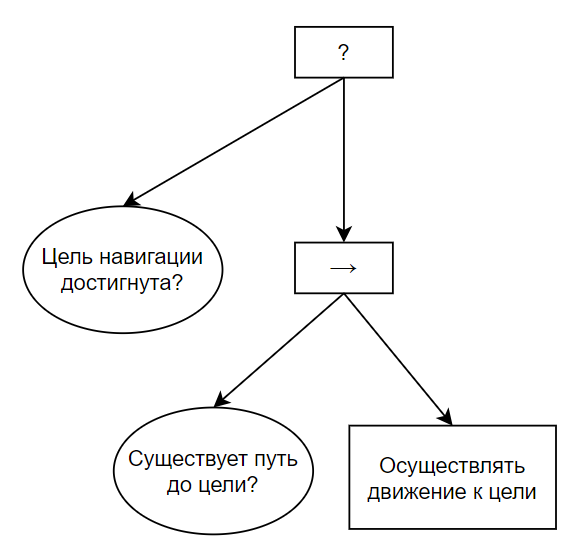
\includegraphics[width=0.5\textwidth]{images/chap_1/bt_example.png}
    \caption{Пример использования поведенческого дерева}
    \label{fig:bt_example}
\end{figure}

Отметим преимущества поведенческих деревьев:
\begin{enumerate}
    \item Модульность - малое число связей между отдельными состояниями. Это дает возможность создавать компоненты независимо друг от друга и встраивать их в систему
    \item Иерархическая структура - действия подразделяются на уровни
    \item Высокая степень реактивности (отзывчивости) - возможность быстро и эффективно реагировать на изменения в среде
    \item Наглядное графическое представление системы
\end{enumerate}

\subsection{Частично наблюдаемые марковские процессы принятия решений}
Марковские процессы принятия решений (МППР) и их дальнейшее развитие в виде частично наблюдаемых марковских процессов принятия решений (ЧНМППР) является еще одним подходом к управлению поведения робота. Их структура похожа на структуру конечных автоматов, однако МППР наделены вероятностными перехода между состояний. 

МППР определяется в виде кортежа $(S, A, T, R)$. Как и у конечного автомата МППР имеет множетсво возможных состояний $S$ и множество стохастических переходов между ними $T$, каждому из которых присвоена некоторая вероятность. Также присутствуют множества действий $A$ и наград $R: S \times A \rightarrow \mathbb{R}$, которые соответствуют действиями. \\
В ходе функционирования робота в среде, оптимизируется функционал, который максимизирует ожидаемую награду, полученную роботом за время действия. В ходе оптимизационной задачи робот находит требуемое поведение $\pi$ \cite{van2012reinforcement}.

Различие между МППР и частично наблюдаемых МППР заключается в том, что текущее состояние системы может быть не опредлено и системе требуется проводить дополнительные наблюдения по которым оценивается вероятность быть в определенном состоянии \cite{krishnamurthy2016partially}. Математически ЧНМППР описывается как кортеж $(S, A, T, R, Z, O)$, где помимо компонент МППР присутствуют также $Z$ - дополнительные наблюдения, а $O$ - это функция вероятности обнаружить $Z$ в состоянии $S$.

\begin{figure}[h]
    \centering
    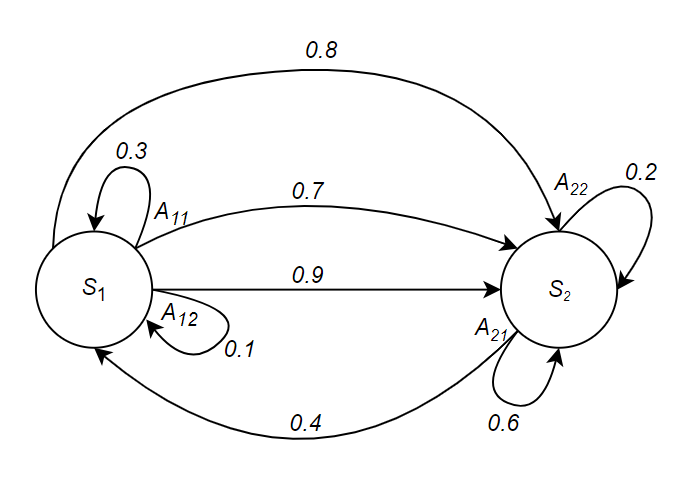
\includegraphics[width=0.75\textwidth]{images/chap_1/pomdp.png}
    \caption{Пример частично наблюдаемого МПР}
    \label{fig:podmp}
\end{figure}

ЧНМППР обычно используются для применения в неопределенном окружении, когда роботу требуется сталкиваться с неизвестными сценариями и подстраивать свое поведение для достижения цели. В основе данной системы принятия решений лежит вероятностный подход, а значит нет никаких гарантий что поведение системы будет детермированным (будет одинаковым каждый раз при одних и тех же условиях), что может быть недопустимых в некоторых областях применения.

\section{Навигация в динамическом окружении}
Для применения методов навигации к условиям динамического окружения требуется модифицировать алгоритмы. Так как в случае наличия динамических объектов в среде требуется каким-то образом учитывать их движение во избежание критических ситуаций \cite{laugier2007autonomous}.

\subsection{Обнаружение динамических объектов}
Для обнаружения динамических объектов в окружении можно применять метод основанный на отделении заднего плана (представляющего статическую карту местности) и переднего плана (динамические объекты) \cite{albers2019online}. Для этого используется представление окружения в виде карты занятости с отмеченными значениями стоимости, которая обрабатывается как изображение в градациях серого. 

Операция выделения переднего плана используется во многих задачах компьютерного зрения, например для распознавания объектов. Существует множество алгоритмов, в данной работы мы рассмотрим метод с низкой вычислительной сложностью, использующий бегущие усредняющие фильтры:

\begin{equation}
    \label{eq:e7}
    F_{t+1}(x,y) = (1 - \alpha)F_t(x,y) + \alpha C_t(x,y),
\end{equation}
где $(x,y)$ - координаты пикселя изображения, $F_t$ - изображение переднего плана в момент времени $t$, $C_t$ - текущее входное изображение карты стоимости в момент времени $t$, $\alpha$ - коэффициент определяющий влияние карты стоимости на результат.

Для более точного выделения переднего плана используется комбинация из двух фильтров (медленный и быстрый) с добавлением медианного фильтра для 8 соседних пикселей:

\begin{equation}
    \label{eq:e8}
    F_f(t+1) = \beta ((1-\alpha_f)F_f(t) + \alpha_f C(t)) + \frac{1 - \beta}{8} \sum_{i \in N} F_{f,i}(t),
\end{equation}
\begin{equation}
    \label{eq:e9}
    F_s(t+1) = \beta ((1-\alpha_s)F_s(t) + \alpha_s C(t)) + \frac{1 - \beta}{8} \sum_{i \in N} F_{s,i}(t),
\end{equation}
где $F_f(t)$ и $F_s(t)$ - изображения переднего плана в момент времени $t$, $\alpha_f$ и $\alpha_s$ - коэффициенты влияний карты стоимости $C(t)$ на выходы фильтров, при чем 
\begin{equation}
    0 \leq \alpha_s \leq \alpha_f \leq 1.
\end{equation}
А коэффициент $\beta$ определяет соотношение между вкладом центральной клетки и влиянием соседних клеток на фильтры.

После применения данных фильтров к каждому пикселю применяется два пороговых фильтра для определения принадлежности пикселя к динамическому объекту:
\begin{enumerate}
    \item Активация быстрого фильтра: $F_f(t) > c_1$
    \item Разница между быстрым и медленным фильтром должна превышать порог $c_2$: $F_f(t) - F_s(t) > c_2$
\end{enumerate}

Результатом этой пороговой операции является бинарная карта, на которой отмечены все динамические препятствия. Далее применяются метод кластеризации с вычислением центров и границ объектов. Для этого успешно применяются методы компьютерного зрения из библиотеки \textit{OpenCV}, например \cite{opencv-blobs}.

\subsection{Слежение за динамическими объектами}
Следующим пунктом реализуется слежение за выделенными объектами на бинарной карте. 

Задача сопоставления объектов во времени является видом задачи о назначении (одна из фундаментальных задач комбинаторной оптимизации), которая решается венгерским алгоритмом \cite{hung-alg}. Алгоритм минимизирует общее евклидово расстояние между центрами уже отслеживаемыми объектами и новым набором центров выделенных объектов. 

Математическая формулировка выглядит следующим образом. Существует матрица стоимостей $C$, элементы которой $C_{i,j}$ определяют стоимость сопоставления ранее отслеженного объекта $i \in A$ с только что обнаруженным объектом $j \in B$. Функция стоимости представляет собой евклидову норму для рассчета расстояния между объектами из двух множеств. Цель оптимизации найти такую конфигурацию пар, которая будет обладать минимальной суммой стоимостей пар, то есть:
\begin{equation}
    min \sum_{i \in A} \sum_{j \in B} C_{i,j} X_{i,j},
\end{equation}
где $X$ - булева матрица выбранных пар.

Теперь произведем оценку положения и скорости динамических объектов. Для решения такой задачи используется фильтр Калмана. \\
Фильтр Калмана - это алгоритм позволяющий оценивать некоторые неизвестные переменные с учетом поступления новых наблюдений с течением времени \cite{kalman1}. Фильтр Калмана оценивает вектор состояния линейных динамических систем в форме вход-состояние-выход. \\
Пусть дана дискретная модель в форме ВСВ:
\begin{equation}
    \begin{cases}
        x_k = A x_{k-1} + B u_{k-1} + w_{k-1}, \\
        y_k = C x_k + \nu_k,
    \end{cases}
\end{equation}
где $A$ - матрица состояний, $B$ - матрица управляющих воздействий, $C$ - матрица наблюдений, $x_k$ - вектор состояний на шаге $k$, $y_k$ - вектор наблюдений на шаге $k$, $u_k$ - вектор управления на шаге $k$, $w_k \sim \mathcal{N}(0, Q)$ - вектор внешних возмущений, $\nu_k \sim \mathcal{N}(0, R)$ - вектор помех измерений.

Фильтр Калмана производит оценку вектора состояния $x_k$ на дискретном шаге $k$ имея вектор начального состояния $x_0$, значения векторов наблюдений $y_1, y_2, y_3, ...$, а также матриц системы $A, B, C, Q, R$.
В процессе работы метода повторяются два шага: 
\begin{enumerate}
    \item Шаг предсказания:
    \begin{enumerate}
        \item Оценка вектора состояния:
        \begin{equation}
            \widehat{x}_k = A \widehat{x}_{k-1} + B u_k
        \end{equation}
        \item Оценка ковариационной матрицы: 
        \begin{equation}
            P_k = A P_{k-1} A^T + Q
        \end{equation}
    \end{enumerate}
    \item Шаг обновления:
    \begin{enumerate}
        \item Невязка вектора измерения:
        \begin{equation}
            \widetilde{y}_k = y_k - C \widehat{x}_k
        \end{equation}
        \item Усиление фильтра Калмана: 
        \begin{equation}
            K_k = P_k C^T (C P_k C^T + R)^{-1}
        \end{equation}
        \item Обновленная оценка вектора состояния: 
        \begin{equation}
            \widehat{x}_{k_{upd}} = \widehat{x}_k + K_k \widetilde{y}_k
        \end{equation}
        \item Обновленная оценка ковариационной матрицы: 
        \begin{equation}
            P_{k_{upd}} = (I - K_k C)P_k
        \end{equation}
    \end{enumerate}
\end{enumerate}


При адаптации фильтра Калмана к задаче слежения за объектами в двумерном пространстве вектор состояния примет вид \cite{saho2017kalman}:
\begin{equation}
    x_k = \begin{bmatrix}
        p_k \\
        v_k
    \end{bmatrix} = \begin{bmatrix}
        p_{k−1} + v_{k−1}dt + \frac{1}{2} \widetilde{a}_{k-1} dt^2 \\
        v_{k-1} + \widetilde{a}_{k-1}dt
    \end{bmatrix},
\end{equation}
где $p$ и $v$ - двумерные векторы положения и скорости в пространстве, $\widetilde{a}$ - ускорение приложенное к объекту.

Матричный вид:
\begin{equation}
    x_k = A x_{k-1} + B \widetilde{a}_{k-1},
\end{equation}
где $\widetilde{a}_{k-1}$ - неизвестный нам сигнал, $A = \begin{bmatrix}
    I_{2\times2} & I_{2\times2}dt \\
    0_{2\times2} & I_{2\times2}
\end{bmatrix}$, $B = \begin{bmatrix}
    \frac{1}{2} I_{2\times2} dt^2 \\ I_{2\times2} dt
\end{bmatrix}$.

В данном методе применяется модель постоянной скорости для объектов, а значит между дискретными шагами $k-1$ и $k$ скорость является константой. \\ 
Исходя из вида вектора состояния, внешние силы ($w$) вызывают постоянное ускорение ($\widetilde{a})$, которое распределено по закону $\mathcal{N}(0, Q)$. \\
Значит ковариационная матрица распределения внешних возмущений:
\begin{equation}
    Q = B B^T \sigma_a^2 = \begin{bmatrix}
        \frac{1}{4} I_{2\times2} dt^4 & \frac{1}{2} I_{2\times2} dt^3 \\
        \frac{1}{2} I_{2\times2} dt^3 & I_{2\times2} dt^2
    \end{bmatrix} \sigma_a^2,
\end{equation}
где $\sigma_a^2 = \begin{bmatrix}
    \sigma_{ax}^2 & \sigma_{ay}^2
\end{bmatrix}^T$ - дисперсия вектора $w$.

Вектор наблюдений состоит только из положения объекта:
\begin{equation}
    y_k = C x_k + \nu_k,
\end{equation}
где $\nu_k$ - вектор помех измерений порождаемый распределением $\mathcal{N}(0, R)$, а матрица вектора измерений $C = \begin{bmatrix}
    I_{2\times2} & 0_{2\times2}
\end{bmatrix}$, $R = I_{2\times2}$ - ковариационная матрица распределения помех измерений.

Начальные значения матрицы $P$ могут быть выбраны следующим образом:
\begin{equation}
    P = \begin{bmatrix}
        I_{2\times2} & O_{2\times2} \\
        O_{2\times2} & 10 \times I_{2\times2}
    \end{bmatrix},
\end{equation}
где ковариация ошибок для скоростей установлена выше, поскольку они не измеряются.

\subsection{Отображение динамических объектов на карте стоимости}
Для того чтобы планировщик пути учитывал информацию о полученной скорости и положении отслеживаемых динамических объектов требуется отметить зоны штрафов вокруг динамических объектов на карте стоимости \cite{yang2019social}.

Значения штрафов вокруг объектов будут распределены по двумерному гауссовскому закону. При этом ковариационная матрица распределения должна иметь такие значения, чтобы область штрафа была больше для более быстрых объектов. Также учитывается направление скорости для отображения большей зоны штрафа вдоль направления движения объекта. Это достигается путем смешивания двух двумерных нормальных распределений.

Итак, имея набор динамических объектов с определенными положением и скоростью относительно глобальной системы координат, для каждого из них проведем следующие операции. \\
Пусть $c(x,y)$ - координаты центра объекта, определяем локальную систему координат с центром в $c$, осью абсцисс сонаправленной с вектором скорости и перпендикулярной ей осью ординат.\\
Тогда область штрафа определяется в виде функции:
\begin{equation}
    \Phi_{c, \sum_{front}, \sum_{back}}(q) = \delta(x_q)\Phi_{c, \sum_{front}}(q) + (1-\delta(x_q))\Phi_{c, \sum_{back}}(q),
\end{equation}
где $q=(x_q,y_q)$ - координаты точки в глобальной системе координат, $\Phi_{c, \sum_{front}}(q)$ - функция Гаусса для зоны штрафа перед объектом, $\Phi_{c, \sum_{back}}(q)$ - функция Гаусса для зоны штрафа позади объекта, $\delta(x)$ - функция параметра для объединения гауссиан:
\begin{equation}
    \delta(x) = \begin{cases}
        1, & \textup{если} \qquad x \geq 0 \\
        0, & \textup{иначе}
    \end{cases}
\end{equation}

Функции Гаусса имеют вид:
\begin{equation}
    \Phi_{c, \sum}(q) = A \exp[-\frac{(\Vert q-c \Vert_2 \cos(\vartheta - \vartheta_c))^2}{2\sigma^2_x} - \frac{(\Vert q-c \Vert_2 \sin(\vartheta - \vartheta_c))^2}{2\sigma^2_y}],
\end{equation}
где $q=(x_q,y_q)$ - координаты точки и $c=(x_c,y_c)$ - координаты центра объекта, $\vartheta$ - угол, образованный вектором положения точки относительно глобальной оси абсцисс, $\vartheta_c$ - угол между направлением движения динамического объекта и глобальной осью абсцисс, $A = 255$ - амплитуда, устанавливается максильным значением карты стоимости, $\sigma^2_x$ и $\sigma^2_y$ диагональные значения ковариационной матрицы $\sum$, которые определяют форму зоны штрафов около объектов. \\
Для двух Гауссиан ковариационные матрицы определяются так:
\begin{equation}
    \sum_{front} = \begin{pmatrix}
        \sigma^2_{x_{front}} & 0 \\
        0 & \sigma^2_{y_{front}}
    \end{pmatrix}; \sum_{back} = \begin{pmatrix}
        \sigma^2_{x_{back}} & 0 \\
        0 & \sigma^2_{y_{back}}
    \end{pmatrix}
\end{equation}
Таким образом, варьируя значения $\sigma^2_x$ и $\sigma^2_y$, можно изменять форму зоны штрафов. 

Также, для учета скорости объекта дисперсии могут быть переопределены следующим образом:
\begin{equation}
    \begin{cases}
        \sigma^2_{x_{front}} = (1+r)\sigma^2_{x_{front}} \\
        \sigma^2_{y_{front}} = (1-\frac{r}{2})\sigma^2_{y_{front}} \\
        \sigma^2_{x_{back}} = (1-r)\sigma^2_{x_{back}} \\
        \sigma^2_{y_{back}} = (1-\frac{1}{4})\sigma^2_{y_{back}} \\
    \end{cases},
\end{equation}
где $r = \frac{v_{cur}}{v_{max}}$ - соотношение текущей скорости и максимальной скорости объекта.

